\chapter[Evaluating Multiallelism for Genomic Prediction Applications in
Potato]{Evaluating Multiallelism for Genomic Prediction Applications in
Potato}
\chaptermark{Evaluating Multiallelism for Genomic Prediction Applications in
Potato}
\label{cha:chapter5}
\vspace*{\fill}

\newpage

% Options for packages loaded elsewhere
\PassOptionsToPackage{unicode}{hyperref}
\PassOptionsToPackage{hyphens}{url}
\PassOptionsToPackage{dvipsnames,svgnames,x11names}{xcolor}
%

\usepackage{amsmath,amssymb}
\usepackage{iftex}
\ifPDFTeX
  \usepackage[T1]{fontenc}
  \usepackage[utf8]{inputenc}
  \usepackage{textcomp} % provide euro and other symbols
\else % if luatex or xetex
  \usepackage{unicode-math}
  \defaultfontfeatures{Scale=MatchLowercase}
  \defaultfontfeatures[\rmfamily]{Ligatures=TeX,Scale=1}
\fi
\usepackage{lmodern}
\ifPDFTeX\else  
    % xetex/luatex font selection
\fi
% Use upquote if available, for straight quotes in verbatim environments
\IfFileExists{upquote.sty}{\usepackage{upquote}}{}
\IfFileExists{microtype.sty}{% use microtype if available
  \usepackage[]{microtype}
  \UseMicrotypeSet[protrusion]{basicmath} % disable protrusion for tt fonts
}{}
\makeatletter
\@ifundefined{KOMAClassName}{% if non-KOMA class
  \IfFileExists{parskip.sty}{%
    \usepackage{parskip}
  }{% else
    \setlength{\parindent}{0pt}
    \setlength{\parskip}{6pt plus 2pt minus 1pt}}
}{% if KOMA class
  \KOMAoptions{parskip=half}}
\makeatother
\usepackage{xcolor}
\usepackage[lmargin=20mm,rmargin=20mm]{geometry}
\setlength{\emergencystretch}{3em} % prevent overfull lines
\setcounter{secnumdepth}{5}
% Make \paragraph and \subparagraph free-standing
\ifx\paragraph\undefined\else
  \let\oldparagraph\paragraph
  \renewcommand{\paragraph}[1]{\oldparagraph{#1}\mbox{}}
\fi
\ifx\subparagraph\undefined\else
  \let\oldsubparagraph\subparagraph
  \renewcommand{\subparagraph}[1]{\oldsubparagraph{#1}\mbox{}}
\fi


\providecommand{\tightlist}{%
  \setlength{\itemsep}{0pt}\setlength{\parskip}{0pt}}\usepackage{longtable,booktabs,array}
\usepackage{calc} % for calculating minipage widths
% Correct order of tables after \paragraph or \subparagraph
\usepackage{etoolbox}
\makeatletter
\patchcmd\longtable{\par}{\if@noskipsec\mbox{}\fi\par}{}{}
\makeatother
% Allow footnotes in longtable head/foot
\IfFileExists{footnotehyper.sty}{\usepackage{footnotehyper}}{\usepackage{footnote}}
\makesavenoteenv{longtable}
\usepackage{graphicx}
\makeatletter
\def\maxwidth{\ifdim\Gin@nat@width>\linewidth\linewidth\else\Gin@nat@width\fi}
\def\maxheight{\ifdim\Gin@nat@height>\textheight\textheight\else\Gin@nat@height\fi}
\makeatother
% Scale images if necessary, so that they will not overflow the page
% margins by default, and it is still possible to overwrite the defaults
% using explicit options in \includegraphics[width, height, ...]{}
\setkeys{Gin}{width=\maxwidth,height=\maxheight,keepaspectratio}
% Set default figure placement to htbp
\makeatletter
\def\fps@figure{htbp}
\makeatother

\usepackage{booktabs}
\usepackage{longtable}
\usepackage{array}
\usepackage{multirow}
\usepackage{wrapfig}
\usepackage{float}
\usepackage{colortbl}
\usepackage{pdflscape}
\usepackage{tabu}
\usepackage{threeparttable}
\usepackage{threeparttablex}
\usepackage[normalem]{ulem}
\usepackage{makecell}
\usepackage{xcolor}
\usepackage{lineno}\linenumbers
\usepackage{pdflscape}
\usepackage[inkscapeformat=png]{svg}
\usepackage{kbordermatrix}
\usepackage{wrapfig}
\usepackage{amsmath}
\DeclareMathOperator*{\argmin}{arg\,min}
\makeatletter
\@ifpackageloaded{tcolorbox}{}{\usepackage[skins,breakable]{tcolorbox}}
\@ifpackageloaded{fontawesome5}{}{\usepackage{fontawesome5}}
\definecolor{quarto-callout-color}{HTML}{909090}
\definecolor{quarto-callout-note-color}{HTML}{0758E5}
\definecolor{quarto-callout-important-color}{HTML}{CC1914}
\definecolor{quarto-callout-warning-color}{HTML}{EB9113}
\definecolor{quarto-callout-tip-color}{HTML}{00A047}
\definecolor{quarto-callout-caution-color}{HTML}{FC5300}
\definecolor{quarto-callout-color-frame}{HTML}{acacac}
\definecolor{quarto-callout-note-color-frame}{HTML}{4582ec}
\definecolor{quarto-callout-important-color-frame}{HTML}{d9534f}
\definecolor{quarto-callout-warning-color-frame}{HTML}{f0ad4e}
\definecolor{quarto-callout-tip-color-frame}{HTML}{02b875}
\definecolor{quarto-callout-caution-color-frame}{HTML}{fd7e14}
\makeatother
\makeatletter
\makeatother
\makeatletter
\makeatother
\makeatletter
\@ifpackageloaded{caption}{}{\usepackage{caption}}
\AtBeginDocument{%
\ifdefined\contentsname
  \renewcommand*\contentsname{Table of contents}
\else
  \newcommand\contentsname{Table of contents}
\fi
\ifdefined\listfigurename
  \renewcommand*\listfigurename{List of Figures}
\else
  \newcommand\listfigurename{List of Figures}
\fi
\ifdefined\listtablename
  \renewcommand*\listtablename{List of Tables}
\else
  \newcommand\listtablename{List of Tables}
\fi
\ifdefined\figurename
  \renewcommand*\figurename{Figure}
\else
  \newcommand\figurename{Figure}
\fi
\ifdefined\tablename
  \renewcommand*\tablename{Table}
\else
  \newcommand\tablename{Table}
\fi
}
\@ifpackageloaded{float}{}{\usepackage{float}}
\floatstyle{ruled}
\@ifundefined{c@chapter}{\newfloat{codelisting}{h}{lop}}{\newfloat{codelisting}{h}{lop}[chapter]}
\floatname{codelisting}{Listing}
\newcommand*\listoflistings{\listof{codelisting}{List of Listings}}
\makeatother
\makeatletter
\@ifpackageloaded{caption}{}{\usepackage{caption}}
\@ifpackageloaded{subcaption}{}{\usepackage{subcaption}}
\makeatother
\makeatletter
\@ifpackageloaded{tcolorbox}{}{\usepackage[skins,breakable]{tcolorbox}}
\makeatother
\makeatletter
\@ifundefined{shadecolor}{\definecolor{shadecolor}{rgb}{.97, .97, .97}}
\makeatother
\makeatletter
\makeatother
\makeatletter
\makeatother
\ifLuaTeX
  \usepackage{selnolig}  % disable illegal ligatures
\fi
\usepackage[style=authoryear,]{biblatex}
\addbibresource{library.bib}
\IfFileExists{bookmark.sty}{\usepackage{bookmark}}{\usepackage{hyperref}}
\IfFileExists{xurl.sty}{\usepackage{xurl}}{} % add URL line breaks if available
\urlstyle{same} % disable monospaced font for URLs
\hypersetup{
  pdftitle={Evaluating Multiallelism for Genomic Prediction Applications in Potato},
  pdfauthor={James Adams, Michiel de Vries, Chaozhi Zheng, \& Fred van Eeuwijk},
  colorlinks=true,
  linkcolor={blue},
  filecolor={Maroon},
  citecolor={Blue},
  urlcolor={Blue},
  pdfcreator={LaTeX via pandoc}}

\ifdefined\Shaded\renewenvironment{Shaded}{\begin{tcolorbox}[breakable, frame hidden, boxrule=0pt, interior hidden, enhanced, borderline west={3pt}{0pt}{shadecolor}, sharp corners]}{\end{tcolorbox}}\fi

\section*{Abstract}

Potato breeding must be improved in order to hasten the release of
higher-yielding and more robust potato varieties. The
development and wider adoption of genetic tools like genomic prediction
depend on high quality and high-throughput genotyping platforms in order
to estimate the genetic value of a candidate. Rapid improvement of the
potato genome sequence and genotyping platforms are both a boon and
problem for breeders as a higher volume of high quality marker data
needs proper methodological applications to make it useful. Of specific
interest to the authors of this paper is the use of multiallelic
marker information, whether identity-by-state (using haplotags, HT) or
identity-by-descent (IBD), and if it offers benefits over that of
biallelic variants (using single nucleotide polymorphisms, SNPs) for the
prediction of genomically estimated breeding values for tuber yield in
potato. Consideration over model choice is also worthwhile given the
hierarchical structure of multiple alleles to a given locus must be
interrogated to ensure a proper representation of the statistical
architecture. We considered traditional shrinkage-based models (ridge
regression, LASSO), group-wise modified models (grouped LASSO), and
advanced kernel approaches (Gaussian Kernel). Using phenotypic and
genotypic data from a hybrid potato breeding program, we found that
multiallelic-based predictors could be used to achieve adequate prediction
accuracy for both IBD (total tuber yield: 0.65 - 0.67) and haplotag
(total tuber yield: 0.71 - 0.75) probesets with the latter being
generally more accurate in total tuber yield, tuber size and dry matter
content. All prediction models using the biallelic probset (SNP) were
the most performant across all traits. Model choice had a
significant impact on prediction accuracy and error with the Transformed
Gaussian Kernel performing best across each trait. These findings
suggest that while multiallelic marker information can offer better
discriminative power in many breeding related applications, this is
not necessarily the case for model-based genetic assessment. To our knowledge, this research represents a first evaluation of multiallelic predictors for genomic prediction applications in
potato.

\hypertarget{introduction}{%
\section{Introduction}\label{introduction}}

Genetic improvement in potato (\emph{Solanum tuberosum}) is a topic
which has garnered much interest in recent decades. It includes issues related to large progeny variances,
choice of propagation systems, significant genotype by environment
interactions, and the fundamental biology of the crop
\autocite{Mendoza1974,Tai1979,Almekinders2009}. For over a century, the
challenges around potato's evolution in particular have come to the
forefront beginning with its notable aversion to inbreeding and
tetrasomic inheritance \autocite{Krantz1924,Swaminathan1954}. It was not
until the advent of technologies like molecular sequencing that the
effects of potato's polyploidization were seen in full with strong
evidence of accumulated deleterious mutations, and genomic variation
more generally
\autocite{Lian2019,Hardigan2016,Marand2019,Kyriakidou2020}. This is
exemplified by a large number of SNPs/indels (1 SNP variant per 29
basepairs) as well as a large quantity of structural variants (over
560,000 in one pan-genome) when sampling the Solanum genepool
\autocite{ThePotatoGenomeSequencingConsortium2011,Tang2022}. This also
extends to important functional regions in potato. Examples include
genes controlling maturity (\emph{stCDF}), tuber shape (\emph{StOFP20}),
and self-incompatibility (\emph{sli})
\autocite{Kloosterman2013,Eck2022,Ames2024}.

The state of functional variation in the Solanum genepool naturally has
implications for genetic applications in potato. Since the release of
the first potato genome, multiple molecular strategies have been
deployed successfully including KASP, microarrays, untargeted
genotyping-by-sequencing (GBS), and recently targeted GBS methods
\autocite{Vos2015,Meijer2018,Wilson2021,Endelman2024}. The latter
approach is especially interesting for potato as it makes marker design
amenable to hyper-variable regions where multiple haplotypes are
present. This is already being leveraged in platforms like PotatoMASH
(Potato Multi-Allele Scanning Haplotags), a targeted amplicon sequencing
strategy which was developed with the express purpose of genetic
discovery in potato \autocite{Leyva-Perez2022}. The fundamental unit of
capture are a group of variants that constitute a short-range
haplotype, or to use the language of \autocite{Tinker2016}, a
\emph{haplotag}. The use of haplotags over traditional SNP variants has
been shown to offer better statistical power in genetic modelling
applications (e.g. GWAS) and have already been used for QTL discovery
for multiple traits in potato including unreduced pollen, tuber eye
depth, and tuber number
\autocite{ThereseNavarro2022,Clot2024,Vexler2024}.

If we want to consider multiallelic effects in potato, haplotags
represent an identity-by-state (IBS) approach where any estimated effect
is based upon the sampled DNA sequence. An alternative to this would be
to infer the ancestral state of that piece of DNA relative to it's
population history. Within population genetics, this is otherwise known as
identity-by-descent (IBD) \autocite{Falconer1996}. Increasing interest
in IBD-based methods have coincided with the emergence of popular
multi-parental population designs such as the NAM or MAGIC which enable
parametrizing genetic models according to multiple founder effects
\autocite{Li2021,Garin2021}. Over the past decade, this interest has
extended from structured balanced pedigrees to that of arbitrary design
thanks to Hidden-Markov based approaches such as those found in RABBIT
\autocite{Zheng2015}. These methods become immediately interesting with
deeper and more complex pedigrees such as those found in breeding
programs \autocite{Tisne2015,VanEeuwijk2010}. Despite interest by
breeders, there are scant studies which have evaluated their feasibility
in a breeding program where strong forces like genetic drift and
selection make breeding populations deviate significantly from these
more idealized multi-parental populations \autocite{Hill2014, Garin2021}.

\begin{tcolorbox}[enhanced jigsaw, opacitybacktitle=0.6, bottomtitle=1mm, colback=white, arc=.35mm, opacityback=0, breakable=false, left=2mm, titlerule=0mm, rightrule=.15mm, toprule=.15mm, colbacktitle=quarto-callout-color!10!white, bottomrule=.15mm, coltitle=black, toptitle=1mm, title={Table 1 Description of four probesets used in hybrid prediction}, leftrule=.75mm]

(Left) The four predictor sets with the number of hybrid observations,
the number of loci, and the
number of predictors derived from each marker type. These include the
original short-sequence based haplotags (HT), identity-by-state single nuclear polymorphisms (SNP), sparse single nuclear polymorphisms (sSNP), and the
founder-derived identity-by-descent variants (IBD or IBDVs). (Right) Diagram of the haplotag model for all 811 probes
used in this study. The amplicon sequence is composed of a 75 base pair
        target region which contains a variable number of distinguishing variants. The haplotag alleles are treated as is while both SNP and IBD datasets are based upon the constituent variants. The IBDVs are then the probability of a variant in question having descended from a given founder line. In this example, this region is heterozygous for founders 2 and 3 for all five variants within the amplicon sequence.

\label{table:1}

\begin{figure}[H]

\begin{minipage}[t]{0.50\linewidth}

{\centering 

\begin{longtable}[]{@{}cccc@{}}
\toprule\noalign{}
ID & Hybrids & Markers & Predictors \\
\midrule\noalign{}
\endhead
\bottomrule\noalign{}
\endlastfoot
HT & 783 & 811 & 2596 \\
SNP & 783 & 2612 & 2612 \\
sSNP & 783 & 1748 & 1748 \\
IBD & 783 & 1748 & 19518 \\
\end{longtable}

}

\end{minipage}%
%
\begin{minipage}[t]{0.50\linewidth}

{\centering 

\raisebox{-\height}{

\includegraphics[width=88mm,height=\textheight]{./figs_05/describe-seqsnp.pdf}

}

}

\end{minipage}%

\end{figure}

\end{tcolorbox}

It is clear that both haplotag and IBD variants have been useful in many
genetic applications in potato \autocite{Korontzis2020,Amadeu2021}.
However, to date, neither have been tested in genome-wide prediction for
diploid or polyploid potato. There has also been little examination at
benefits of IBD marker information over that of IBS when both leverage multiallelism. We therefore consider germplasm from a diploid potato
hybrid breeding program to examine the following questions: (1) Whether
multiallelic markers are more informative then their biallelic
counterparts, (2) Are there statistical model paradigms which better
exploit the multiallelic markers, and (3) whether IBD markers are more
useful over IBS markers in a hybrid breeding schema. We interrogate
these questions using a targeted GBS amplicon platform to derive
haplotags (HT), SNP variants (SNP), estimated IBD profiles (IBD), and a
SNP subset (sSNP) to evaluate benefits of a particular marker paradigm
(See Table 1). We investigate popular shrinkage based methods
(e.g.~ridge regression, LASSO, Kernel regression) as well as group-wise
models for the multiallelic markersets (group-LASSO). We measure the
impact of marker and model choice in a hybrid breeding scenario where we
predict F1 yield performance for several tuber traits in potato
seedlings (Figure \ref{fig-breed}). Similar to previous studies
\autocite{Adams2023}, we restrict ourselves to three important yield
components in potato for genetic interrogation, i.e., total tuber yield
(TY), average tuber volume (TV), and tuber dry matter content (DM).

\begin{figure}
  \begin{center}
    \includegraphics[width=65mm,height=70mm]{./figs_05/describe-breeding.pdf}
  \end{center}
  \caption{Diagram of a simple hybrid breeding schema with founder lines (FLs) at pedigree origin, descendent parent lines (PLs) at the crossing block and derived hybrid crosses (F1).}
  \label{fig-breed}
\end{figure}

\hypertarget{material-methods}{%
\section{Material \& Methods}\label{material-methods}}

\hypertarget{phenotypic-description}{%
\subsection{Phenotypic Description}\label{phenotypic-description}}

For this study, we utilized data from an active hybrid breeding program
(Figure \ref{fig-breed}). We used 1,038 F1 hybrids created from
intercrossing of 554 parent lines. These lines were developed through
pedigree selection of an initial inter-crossing of founder lines
followed by subsequent rounds of selfing, and strong selection pressure
\autocite{Lindhout2011}. These hybrids were evaluated in four yield
trials in 2019 and 2020, all of which were true potato seed (TPS)
transplants. These four trials have been described in full in
\autocite{Adams2023} with the same spatial modelling strategy leveraged
here to derive the best linear unbiased predictions
(BLUPs) for each hybrid over all trials. We chose three phenotypes which
demonstrated consistent heritabilities in this population. This included
tuber dry matter content (DM), average tuber volume (TV), and total
tuber yield (TY). These BLUPs were then used in the following phenotypic
model:

\[\tilde{y} = \mu + g_i + g_j + s_{ij} + \varepsilon_{ij}\]

where \(\tilde{y}\) is the hybrid BLUP, \(\mu\) is the across-trial
mean, \(g_i\) and \(g_j\) are the general combining abilities of the
maternal and paternal lines \(i\) and \(j\), respectively, \(s_{ij}\) is
the specific combining ability of those parents, and
\(\varepsilon_{ij}\) is the residual of that cross. The general and
specific combining abilities were treated as random effects and
considered IID
(\(g \sim \mathrm{N(0,~}\sigma^2_{gca})~~~s \sim \mathrm{N(0,~}\sigma^2_{sca})\)).
The pooled residual variance across the four trials was used to estimate the residual variance (\(\sigma^2_{\varepsilon}\)). From this model, we
extracted GCAs and variances for later reference
(Figure~\ref{tbl-variances}).



\hypertarget{marker-analysis}{%
\subsection{Marker Analysis}\label{marker-analysis}}

Using the dataset described in \autocite{Adams2023}, marker data was
collected on 416 of the original 554 parental lines along with 13
founder lines which gave rise to this population. These lines were
genotyped with a targeted genotyping-by-sequencing technology (SeqSNP)
developed by LGC \autocite{LGC2019} which included 811 targeted probes
with a varying number of haplotypes per haplotag locus (on average, 6 haplotypes per
haplotag). All other marker predictors were derived from these haplotag sequences (HT). Variants were extracted from the HTs for the 416 inbred
lines resulting in 2612 SNP predictors which became our IBS SNP probeset. Basic variant filtering was performed
on the SNP set including minor allele frequency
(\(\text{maf} \ge 0.05\)) and missingness (\(\text{miss} \le 0.1\)) with
mean imputation performed on missing calls.

These 2612 SNPs together with their pedigree were then used to estimate
identity by descent (IBD) profiles with respect to the 13 genotyped
founders. This was done using a Hidden Markov Modelling framework,
RABBIT, a modular genetics software implemented in Julia with linkage
map, marker quality control, simulation, and other genetic facilities
\autocite{Zheng2015}. We constructed a simple analytical pipeline
composed from three function calls beginning first with
\texttt{magicfilter} followed by \texttt{magicimpute}, and finally
\texttt{magicreconstruct} using the forward-backward algorithm. At model
convergence, we assessed the haplotype probabilities (i.e.~The
probability of a founders' DNA at a given locus), and removed regions of
low confidence (\(p < 0.5\)). Lastly, we derived the expected founder
allele dosage in the hybrid from their parental haplotype expectations
(\(\mathrm T\)) and the pedigree design matrix (\(\mathrm Z\)) through
simple matrix multiplication (\(\mathrm{ZT}\)). In our analysis, we
found evidence of increased sparsity in specific regions,
particularly on chromosome's 1 and 5 (Supplementary Section 1.). This complicated any
comparison of the IBD and SNP datasets as any difference in model
performance could now be the product of ascertainment bias
\autocite{Heslot2013}. To ensure that our evaluation of IBD-based
predictors was valid, we filtered on those SNP variants which passed
through both RABBIT's quality control and post-pipeline filtering.
This marker sparse SNP markerset (sSNP) was was then tested allowing for a proper comparison to the IBD set.

Both SNP and sSNP predictors were encoded by their minor allele dosage
\{AA = 0, Aa = 1, aa = 2\} with each site centered around zero by
subtracting \(2p_i\). However, for both multiallelic datasets (HT and
IBD) we used the additive multi-allelic encoding prescribed by
\autocite{Da2015} and \autocite{Schaid2004} for the genetic partitioning
of multi-allelic genotypes. First, an incidence matrix was constructed from the
genotypes, or what is often referred to as \emph{one-hot encoding} in
the machine learning literature. Because we were only interested in
estimating the \(h - 1\) allelic effects for each locus (otherwise the
model would be over-specified), incidences of the most predominant
allele were removed. We then took twice the allelic frequency of each
haplotype at each locus and subtract the allelic dosages from it to
center each predictor around zero (See Supplementary Section 2). Hybrid allele and haplotype dosages
for SNP, sSNP, and HT markersets were constructed analogously to the IBD
set with the parent allele dosages and pedigree design matrix. In the
end, we were left with four different marker sets for testing (Table 1).

\hypertarget{statistical-modeling}{%
\subsection{Statistical Modeling}\label{statistical-modeling}}

To evaluate the general benefits of multiallelic information, we tested
multiple modelling frameworks. All models here are extensions of
the standard shrinkage-based methods where we regress our hybrid
performance directly on some set of predictors
(\(\tilde{y} = \mathrm{X}\beta + e\)). The only difference lies in how
\(\beta\) was estimated and the contents of \(\mathrm{X}\). Beginning
with the simplest, we conducted a ridge regression based analysis where
the solution for \(\beta\) (i.e.~our allele substitution effects) are found
with:

\[\argmin_{\beta} ||y - \mathrm{X}\beta||^2_2 + \lambda ||\beta||^2_2\]

This is tantamount to ordinary least squares (OLS) with the addition of
a shrinkage parameter (\(\lambda\)) with \(L_2\) regularization on
\(\beta\). A popular alternative to ridge regression is the least
absolute shrinkage and selection operator, or the LASSO:

\[\argmin_{\beta} \frac{1}{2} ||y - \mathrm{X}\beta||^2_2 + \lambda  ||\beta||_1\]

It deviates from the ridge only in the extra \(\ell_1\) penalty on \(\beta\)
which is equivalent to \(\sum^p_i |\beta_i|\). This ensures that some predictors are selected while others are fixed to 0. For both ridge regression and LASSO models, we used the
\texttt{glmnet} R package which invokes an elastic net approach where
the ridge (\(\alpha = 1\)) and lasso (\(\alpha = 0\)) are special cases
of a general bridge model \autocite{Friedman2010}.

Because our IBD and HT predictors have an inherent biological structure
between them, it would be worthwhile to have it reflected in the model
as well. If there is a particular region or gene which has some
effect on a phenotype, it would be useful to group all alleles for that
locus. One effective approach for this would be the group Lasso
\autocite{Ogutu2014}. Adapting the same notation from above, the group
LASSO can be expressed as:

\[\argmin_{\beta} \frac{1}{2} ||y - \mathrm{X}\beta||^2_2 + \lambda \sum_{\mathscr{j} = 1}^J \sqrt{p_j}||\beta_j||_2\]

where the \(\ell_1\) penalty has been replaced with an \(\ell_2\)
penalty for each group of alleles at a locus \(j\) multiplied by the
square root of the number of alleles at that site (\(\sqrt{p_j}\)).
Estimation of the HT and IBD allelic effects
was done using the \texttt{gglasso} R package \autocite{Yang2015}. Estimated parameters were measured for all LASSO models (See Supplementary section 3).

The last predictive method we tested was the Gaussian Kernel framework
proposed by \autocite{Perez-Elizalde2015}. The primary motivation was to
evaluate if the construction of a kernel with multiallelic marker
information better captures cryptic epistasis which could benefit
genome-wide prediction. The transformed Gaussian Kernel estimates the
joint distribution for the bandwidth and form parameters through a
Markov Chain Monte Carlo (MCMC) Gibbs sampler. The bandwidth parameter
is central in the estimation of the Gaussian Kernel and the form
parameter is essentially equivalent to the inverse of the shrinkage
parameter used in earlier models. We adapted the scripts provided by
\autocite{Perez-Elizalde2015} with a total MCMC iterations of 77,000 and
a burn-in of 2,000. Sampled parameter posterior distributions were also collected for each trait (See Supplementary section 4).

\hypertarget{model-evaluation}{%
\subsubsection{Model evaluation}\label{model-evaluation}}

All model paradigms and predictor types were tested with a simple 5-fold
cross-validation procedure with 50 replications. The same folds were
used across tested models for valid comparisons across each run. Because
we were assessing the accuracy of models which were extensions of the linear model, we used traditional model
performance statistics \autocite{Hsu2017}. These include the prediction
accuracy (Pearson correlation coefficient), statistical bias (the
regression coefficient of the across-trial hybrid BLUP on its predicted value
\(\beta_{\tilde{y}, \hat{y}}\)), and the per cent root mean square error
of prediction
(\(100 \times \sqrt{\mathrm{E}\left ((\tilde{y} - \hat{y}) ^ 2 \right )} / \mu\))
where each error is scaled by the trait mean. All measures for model
performance are provided for each tuber trait studied here
(Figure~\ref{tbl-summaries}).

\hypertarget{results}{%
\section{Results}\label{results}}

Using the same BLUPs for the 1,038 hybrids of the multi-environment
trial datasets from \autocite{Adams2023}, we were able to estimate the
genetic variance and pooled residual variance for these three traits
(Figure~\ref{tbl-variances}). All heritibalities were high with average
tuber volume being the highest among the three variates. From this model
we were also able to estimate general combining abilities for the 416
parental lines used in the hybrid crossing block. Because some parental
lines were not genotyped, a significant fraction of hybrids were
excluded from subsequent analysis. Therefore, 783 hybrids were retained
for IBD triage and genetic modelling.

\begin{figure}

\begin{minipage}[t]{\linewidth}

{\centering 

\hypertarget{tbl-variances}{}
    \caption{\label{tbl-variances}The full genetic variance (\(2\cdot \sigma^2_{gca} + \sigma^2_{sca}\)), pooled residual variance, and
heritability for dry matter content (DM), average tuber volume (TV), and
total tuber yield (TY) along with the distribution of predicted general
combining abilities (GCAs) for each. The +1/-1 standard deviations of
the GCAs are given for each trait. }\tabularnewline

\centering
\begin{tabular}{lrrr}
\toprule
Trait & \(\sigma^2_G\) & \(\sigma^2_{\varepsilon}\) & \(H^2\)\\
\midrule
DM & 2.49 & 0.78 & 0.76\\
TV & 38.31 & 5.18 & 0.88\\
TY & 23.80 & 4.88 & 0.83\\
\bottomrule
\end{tabular}

}

\end{minipage}%
\newline
\begin{minipage}[t]{\linewidth}

{\centering 

\includegraphics{./figs_05/unnamed-chunk-3-1.pdf}

}

\end{minipage}%

\end{figure}

The RABBIT pipeline converged providing
haplotype profiles for all 416 inbred lines. Founder composition per
inbred was quite variable, however, a core of founder backgrounds was
observed. Observing the IBD profile for parent line's PL960 and PL314
(bottom and top 1\% percentiles for average tuber volume GCA), they
appeared to share a common core composed of founder line's FL1, FL2, and
FL3. Differential founder contribution between these two inbreds was
also observed with large contributions of founder FL5 in PL960 on
chromosome's 1, 2 and 5, and large contributions of founder FL4 in PL314
on chromosome's 4, 9, 10, 11, and 12. It is also worth noting the large
chromosome blocks with little to no recombination appeared to have
occurred since initial founder crossing. This was most apparent on
chromosome 11 in both inbreds which inherited two different founder
backgrounds.

\begin{figure}

{\centering \includegraphics{./figs_05/fig-ibd-1.pdf}

}

\caption{\label{fig-ibd}The genome-wide identity by descent profiles of
(a) the best parental line (``PL314'') and (b) the worst parental line
(``PL960'') with respect to average tuber volume.}

\end{figure}

\begin{figure}

{\centering \includegraphics{./figs_05/fig-pa-1.pdf}

}

\caption{\label{fig-pa}Median prediction accuracy for dry matter content
(DM), average tuber volume (TV), and total tuber yield (TY) over all
models including ridge regression (RR), LASSO (LS), group LASSO (GLS),
and the Gaussian Kernel (GK) as well as over each predictor type
including short range haplotypes (HT), founder identity by descent
probabilities (IBD), SNPs (SNP), and a sparse SNP set (sSNP). The best
model within predictor type is given in bold while the best model across
predictors is underlined.}

\end{figure}

Looking to predictive performance of our various markerset types, we
found that the SNP-based datasets performed the best across traits and
were particularly superior using the transformed Gaussian Kernel
method (Figure~\ref{fig-pa}). Generally, the HT markerset was less
performant than SNP and sSNP, but these differences were negligible
especially in dry matter content. Additionally, we found very little
difference between the ridge regression and LASSO models. The IBD
probeset consistently under-performed with respect to prediction
accuracy regardless of model or trait tested. We saw minor improvement
between the LASSO and grouped LASSO for the IBD predictors, but this was
only observed in dry matter content. Considering also the prediction
error, the Gaussian Kernel models had consistently the lowest error for
all trait predictor combinations with exception of the grouped LASSO in
drymatter content (Table~\ref{tbl-summaries}). Differences in predictive
bias appeared to be negligible aside from higher rates detected in the
LASSO models, but this was generally to be expected.

\hypertarget{tbl-summaries}{}
\begin{table}
\caption{\label{tbl-summaries}Prediction Accuracy (PA), prediction bias and the per cent root mean
square error (RMSE) for dry matter content (DM), average tuber volume
(TV), and total tuber yield (TY). This was done over all models
including ridge regression (RR), LASSO (LS), group LASSO (GLS), and the
Gaussian Kernel (GK) as well as over each predictor type including short
range haplotypes (HT), founder identity by descent probabilities (IBD),
SNPs (SNP), and a sparse SNP set (sSNP). The best model within predictor
type is given in bold while the best model across predictors is
underlined. }\tabularnewline

\centering
\begin{tabular}{llllllllll}
\toprule
\multicolumn{1}{c}{ } & \multicolumn{3}{c}{DM} & \multicolumn{3}{c}{TV} & \multicolumn{3}{c}{TY} \\
\cmidrule(l{3pt}r{3pt}){2-4} \cmidrule(l{3pt}r{3pt}){5-7} \cmidrule(l{3pt}r{3pt}){8-10}
Model & PA & Bias & RMSE & PA & Bias & RMSE & PA & Bias & RMSE\\
\midrule
\addlinespace[0.3em]
\multicolumn{10}{l}{\textbf{SNP}}\\
\hspace{1em}RR & 0.74 & \textbf{1.01} & 5.78 & 0.76 & \textbf{1.00} & 16.60 & 0.74 & 1.01 & 22.85\\
\hspace{1em}LS & 0.74 & 0.90 & 5.80 & 0.76 & 0.88 & 16.89 & 0.74 & 0.95 & 22.86\\
\hspace{1em}GK & \underline{\textbf{0.75}} & 1.02 & \underline{\textbf{5.68}} & \textbf{0.78} & 0.98 & \textbf{15.90} & \underline{\textbf{0.76}} & \underline{\textbf{1.00}} & \underline{\textbf{21.97}}\\
\addlinespace[0.3em]
\multicolumn{10}{l}{\textbf{sSNP}}\\
\hspace{1em}RR & 0.73 & \textbf{1.01} & 5.80 & 0.76 & \underline{\textbf{1.00}} & 16.55 & 0.73 & 1.01 & 23.07\\
\hspace{1em}LS & 0.74 & 0.91 & 5.83 & 0.77 & 0.89 & 16.68 & 0.73 & 0.96 & 23.26\\
\hspace{1em}GK & \textbf{0.75} & 1.01 & \textbf{5.69} & \underline{\textbf{0.79}} & 0.99 & \underline{\textbf{15.77}} & \textbf{0.76} & \textbf{1.00} & \textbf{22.15}\\
\addlinespace[0.3em]
\multicolumn{10}{l}{\textbf{HT}}\\
\hspace{1em}RR & 0.73 & \textbf{1.02} & 5.87 & 0.75 & \textbf{1.00} & 17.09 & 0.72 & \textbf{1.00} & 23.54\\
\hspace{1em}LS & 0.73 & 0.93 & 5.85 & 0.74 & 0.88 & 17.57 & 0.71 & 0.89 & 23.98\\
\hspace{1em}GLS & 0.72 & 0.98 & 5.91 & 0.73 & 0.96 & 17.50 & 0.71 & 0.96 & 23.97\\
\hspace{1em}GK & \textbf{0.74} & 1.03 & \textbf{5.71} & \textbf{0.77} & 0.98 & \textbf{16.43} & \textbf{0.75} & 1.01 & \textbf{22.56}\\
\addlinespace[0.3em]
\multicolumn{10}{l}{\textbf{IBD}}\\
\hspace{1em}RR & 0.65 & \underline{\textbf{0.99}} & 6.48 & 0.71 & \textbf{1.01} & 18.12 & 0.65 & \textbf{1.00} & 25.73\\
\hspace{1em}LS & 0.65 & 0.81 & 6.66 & 0.70 & 0.86 & 18.45 & 0.67 & 0.88 & 25.46\\
\hspace{1em}GLS & \textbf{0.67} & 0.94 & \textbf{6.36} & 0.70 & 0.91 & 18.31 & \textbf{0.67} & 0.88 & 25.36\\
\hspace{1em}GK & 0.67 & 1.04 & 6.38 & \textbf{0.71} & 1.03 & \textbf{18.02} & 0.67 & 1.05 & \textbf{25.25}\\
\bottomrule
\end{tabular}
\end{table}

\hypertarget{discussion}{%
\section{Discussion}\label{discussion}}

Examining the first from our set of questions, the biallelic-based
predictors (both SNP and sSNP probesets) exhibited the greatest
modelling accuracy within our cross-validation schema and were stable
across statistical models (Figure~\ref{fig-pa}). The lack of significant
differences between the SNP and sSNP probesets suggest that differences in model performance due to
genome coverage are negligible between 2600 and 1700 SNPs. Taking this further, the
increased prediction error observed with the IBD predictor set then was
not the product of ascertainment bias of filtered regions, but rather the
information content of the haplotypes themselves (Table~\ref{tbl-summaries}). In contrast to
our IBD set, our haplotag-based set of predictors performed generally
better and were nearly identical to the other predictor types; this was most
apparent for tuber dry matter content (Figure~\ref{fig-pa}). This poses
an interesting question of why the HT set is generally identical across
models for dry matter content but not so for other traits. One potential
explanation could be that the statistical architecture, or \emph{genetic
complexity}, of dry matter content is less than that of the other yield
components can be generalized well by both the HT and SNP/sSNP probesets
in contrast to yield components like tuber volume and gross yield.
Additionally, the prediction of tuber volume or total tuber yield could
be improved by a haplotag parameterization which considers the
relationship of alleles within a locus. One potential solution could to
integrate the structural distance between haplotag alleles into a
variance-covariance matrix for each haplotype effect
\autocite{Schaid2004}.

\begin{figure}

{\centering 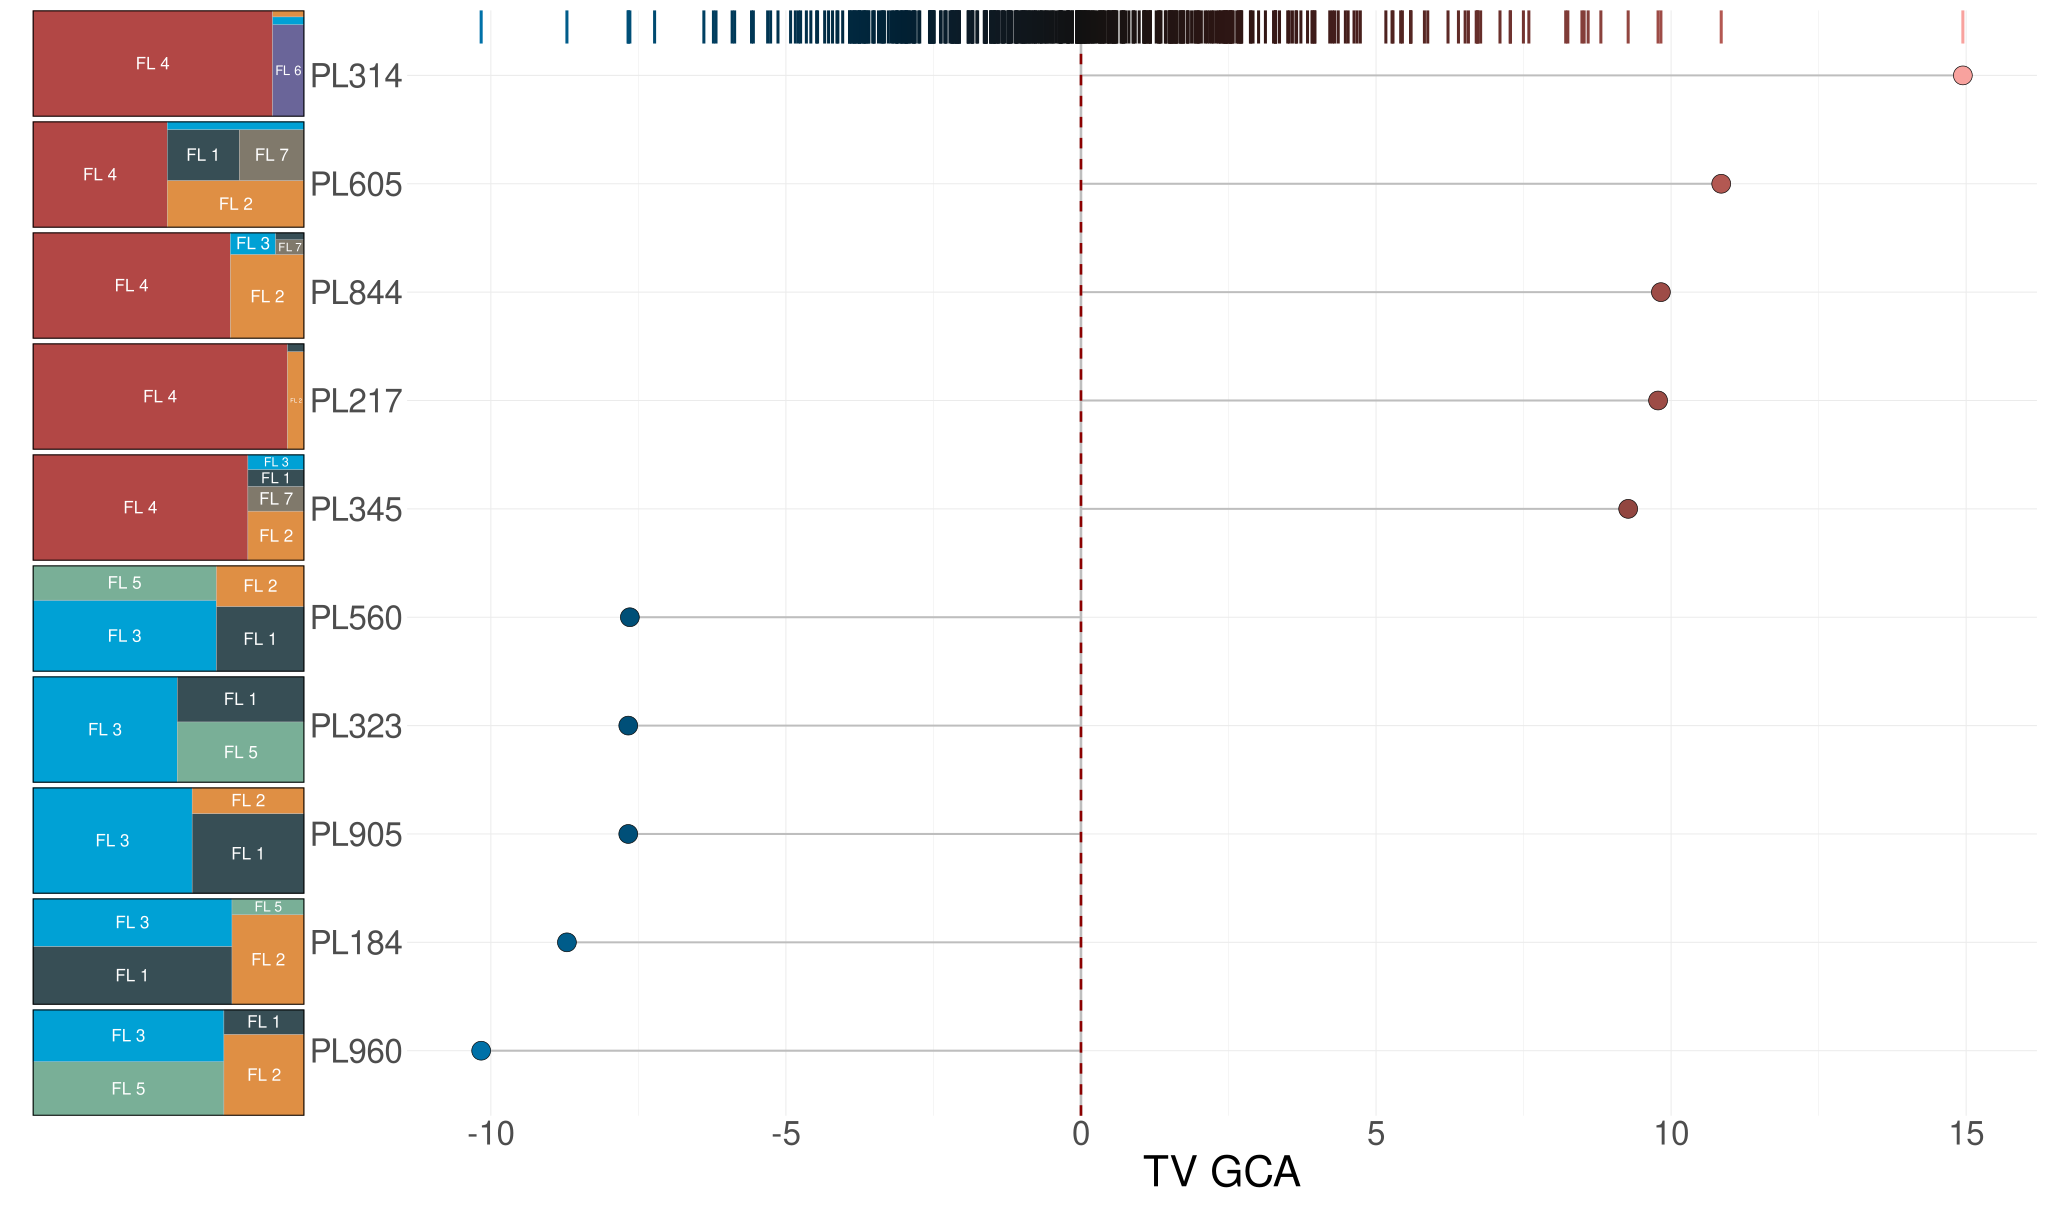
\includegraphics{./figs_05/fig-gca-1.pdf}

}

\caption{\label{fig-gca}The founder origin composition and general
combining ability of the top five and worst five performing parental
lines with respect to average tuber volume (TV). Distribution of all
predicted general combining abilities are provided as a reference.}

\end{figure}

Turning to our second question, there were a few findings with respect
to model choice. For our three tuber characteristics, there was very
little difference between the ridge regression and LASSO models with
exception of a slight increase in prediction bias in the latter
(Table~\ref{tbl-summaries}). For almost all trait and predictor types,
the Gaussian Kernel performed best minimizing the prediction error with
exception of the IBD predictors for dry matter content. The stable
performance of the Gaussian Kernel across traits is worth highlighting
as this has been observed in other crops as well. Whether frequentist
\autocite{Endelman2011} or Bayesian \autocite{Gianola2008}, reproducing
Kernel Hilbert space's are flexible and allow for trait-specific tuning
outside a general variance component. Moreover, kernel-based methods are
even competitive with deep learning methods which continue to gain
popularity in the GP/GS space \autocite{Crossa2019}. We were also
particularly interested in whether grouped-penalization methods could
better exploit the probe and allele structure in the haplotag and IBD
probesets. However, no benefit was observed between the group LASSO and
LASSO with exception of the aforementioned IBD predictors for dry matter
content. There, the group LASSO performed best with respect to the
accuracy and total error. Having said this, the difference observed
between the group LASSO and Gaussian Kernel were negligible.

Touching on the final question, IBD-based predictors performed worse
than their IBS counterparts in the SNP, sSNP, and HT probesets. To
interrogate potential causes, there are multiple explanations. First is the problem of founder choice and which stage of
a breeding program you want to consider the \emph{founding} generation.
While perhaps obvious to the reader, there should be sufficient marker
variation (i.e.~variation via IBS) between founders in order to both
estimate IBD-based origin and in order for it to be useful in genetic
applications. Simulation studies confirm that the benefits of IBD-based
marker effects are most pronounced when there is sufficient marker
diversity in the founding population \autocite{ThereseNavarro2022}. Not
only does marker variation need to be present, but there must also be
relevant \emph{genetic} variation for the model to pick up on. Studies
in barley have shown that when the QTL effects are nearly identical
among founders, modelling on founder effects will not yield benefits
over that of simpler IBS formulations \autocite{Maurer2016,Maurer2017}.
So in order to maximize the utility and accuracy of IBD information in a
breeding program, we would need to identify the generation which offers
the greatest genetic contrast among some set of intermediate genotypes.
There could be alternatives to this through certain pre-processing
methods such as structuring founder effects by the genetic relationship
of the founders (via IBS or IBD) or even transforming these effects
through spectral decomposition as recommended by
\autocite{VanEeuwijk2010}. However, this leads to issues of
interpretability of the estimated parameters. Several population-specific factors such as a early selection intensities might also be related to the underperformance of the IBD probset in
our genome-wide prediction scenario.

Regardless of whether multiallelic data are used in a statistical model,
its utility in a breeding program is not bound there. Extending our example from Figure~\ref{fig-ibd} to include the 5\textsuperscript{th} and 95\textsuperscript{th} percentiles for tuber volume GCA, we can examine their founder line composition (Figure~\ref{fig-gca}).
Evidently, those parental lines with larger tuber volume GCAs tend to
be over-represented by the founder FL4 while those parental lines with
the smallest tuber volume GCA appear to share large compositions of
founders' FL3 and FL5. While the IBD information was not able to
offer any benefits in the context of GP/GS, this does not mean it is
unable to express insight to a breeder regarding their material.
Genome-wide prediction is crucial for informed selection and advancement
of germplasm, but there is still information which influences decision
making even if it does not enter the linear mixed model. Activities like breeding strategy development (e.g.~maintaining breeding pool genetic variance) or breeding cycle evaluation (e.g.~evaluating the impact of previous selection cycles) could both benefit with the introduction of IBD information.

\hypertarget{conclusion}{%
\section{Conclusion}\label{conclusion}}

As potato breeding progresses through the \emph{big-data} era, it is
crucial for geneticists and breeders to assess which information best
informs them of a candidate's genetic potential. With regard to
molecular technologies, the primary questions ought to focus on adequacy
of a marker platform for a specific segment or program along with
whether it is an appropriate choice given the crop's genomic complexity.
Next then, is how that technology could best be leveraged to predict
genetic value, whether it be a simple monogenic target like biotic
resistance or a traditionally complex trait such as yield fractions. The
key findings of this paper suggest that SNP variants are sufficient for
genome-wide prediction in hybrid potato. The use of multi-allelic marker
information such as our haplotag probeset are also possible and offer a
unified prediction approach with a powerful genotyping strategy.
IBD-based predictors also succeeded in the prediction of hybrid yield,
though with a noticeable penalty. Future work should consider further
modelling strategies and alternative parameterisations for multi-allelic
probesets (whether IBS or IBD) to ensure marker information is used
efficiently.




